\documentclass{article}
\usepackage[spanish]{babel}
\usepackage{fancyhdr}
\usepackage{graphicx}
\usepackage{setspace}
\usepackage[table]{xcolor}
\usepackage{tabularx}
\usepackage{array}
\usepackage{multirow}
\usepackage[margin=2.5cm]{geometry}
\usepackage{hyperref}

\pagestyle{fancy}
\lhead{\begin{picture}(0,0) \put(0,-8){
\includegraphics[width=20mm]{img/logoFips.png}} \end{picture}}
\rhead{\begin{picture}(0,0) \put(-25,10){
\includegraphics[width=8mm]{./img/logoAbet.png}} \end{picture}}
\renewcommand{\headrulewidth}{0.5pt}


\fancyhead[C]{
 	\tiny Universidad Nacional de San Agustin de Arequipa \\
  	Facultad de Ingenieria de Produccion y Servicios \\
  	Departamento de Ingenieria de Sistemas e Informatica \\
  	Escuela Profesional de Ingenieria de Sistemas \\
  	\textbf{Programacion Web}
}

\begin{document}
\setstretch{0.75}


\begin{center}
	\Huge \textbf{\\  \Large Laboratorio 02 \\ \Large Tema: Git y GitHub}
\end{center}


\begin{figure}[htbp]
  \centering
  
\includegraphics[width=0.4\textwidth]{img/logoUnsa.png}
\end{figure}


\noindent
\renewcommand{\arraystretch}{2}
\begin{table}[h]
\centering
\begin{tabular}{|c|c|c|c|c|c||}
\hline
\multicolumn{1}{|c|}{\textbf{\scriptsize CURSO:}} & \multicolumn{5}{|c|}{\small Programación Web 2} \\ \hline
\multicolumn{1}{|c|}{\textbf{\scriptsize TÍTULO DE LA PRÁCTICA:}} & \multicolumn{5}{|c|}{\small Git y GitHub} \\ \hline
\multicolumn{1}{|c|}{\textbf{\scriptsize NRO DE PRÁCTICA:}} & \multicolumn{1}{|c|}{\small 2}& \multicolumn{1}{|c|}{\textbf{\footnotesize AÑO:}} & \multicolumn{1}{|c|}{\small 2024-A} & \multicolumn{1}{|c|}{\textbf{\footnotesize SEMESTRE:}} & \multicolumn{1}{|c|}{\small I Semestre} \\ \hline \multicolumn{1}{|c|}{\textbf{\scriptsize ESTUDIANTE:}} & \multicolumn{5}{|c|}{\small Nina Calizaya Rafael Diego} \\ \hline  \multicolumn{1}{|c|}{\textbf{\scriptsize DOCENTE:}} & \multicolumn{5}{|c|}{\small Ing. Lino Pinto} \\ \hline
\end{tabular}
\end{table}

\clearpage
\begin{center}
	\Huge \textbf{\\ \Large Resolución de la Práctica \\}
\end{center}


\section{Entregables}

\subsection{URL al directorio específico del laboratorio en su repositorio GitHub:}
\url{https://github.com/DrN25/pw2_24a/tree/main/Lab02}

\subsection{Commits realizados:}



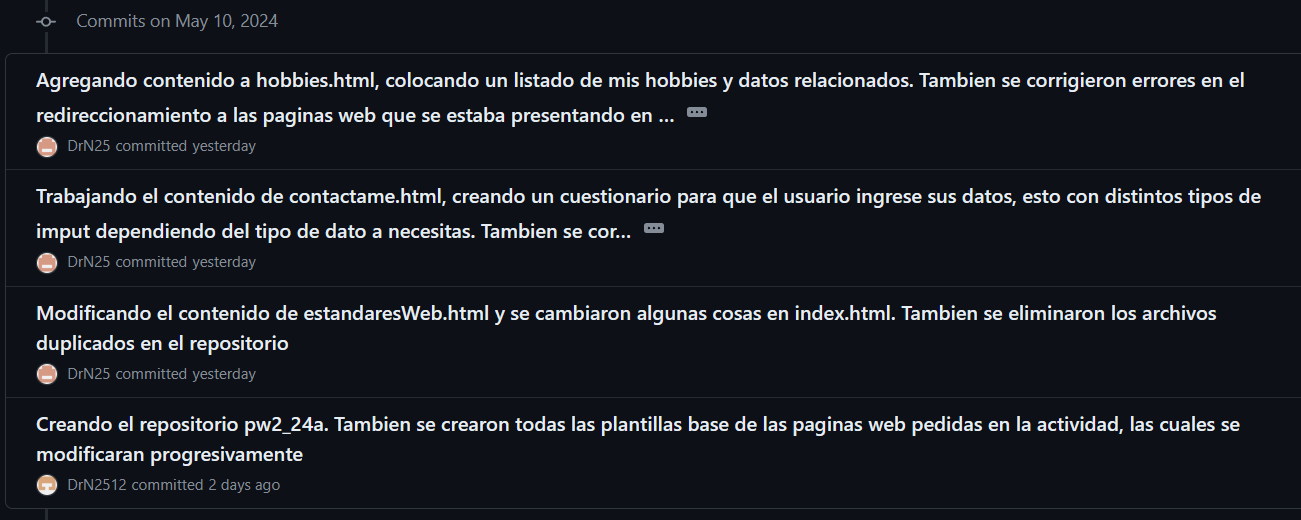
\includegraphics[width=\textwidth]{img/1.png}




\includegraphics[width=\textwidth]{img/2.png}



\subsection{Agregar la estructura de directorios y archivos de su laboratorio hasta el nivel 4.}



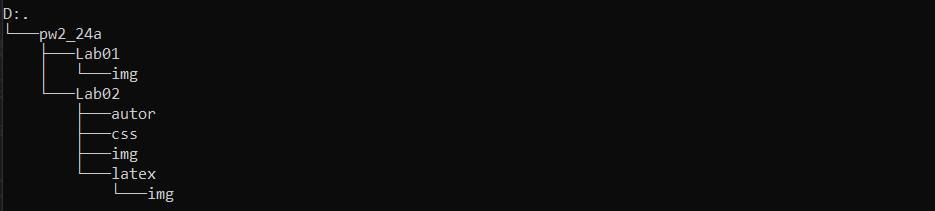
\includegraphics[width=\textwidth]{img/3.png}



\section{Rúbrica}



\includegraphics[width=\textwidth]{img/4.png}

\end{document}

